\chapter{Enfoque propuesto}

El enfoque propuesto para la tesis de exploración coordinada multi-VANT se centra en el desarrollo de un sistema autónomo que emplea varios Vehículos Aéreos No Tripulados (VANTS) para explorar y mapear entornos desconocidos de manera coordinada. Después de identificar técnicas y algoritmos relevantes, seguido del diseño detallado del sistema y su implementación en un entorno simulado.

El diseño e implementación de un sistema autónomo que integre estas tecnologías avanzadas permite abordar los desafíos inherentes a la exploración coordinada con múltiples VANT y complementado con una distrubución de tareas descentralizado.

En resumen, el enfoque propuesto aborda el desafío de la exploración coordinada multi-VANT mediante la integración de algoritmos avanzadas y la evaluación práctica de su desempeño en diferentes ambientes.


%\section{Revisión de la literatura}

%Realizar una revisión exhaustiva de la literatura sobre técnicas y algoritmos existentes para la exploración coordinada con múltiples VANT. Esto incluiría investigar enfoques de planificación de trayectorias, técnicas de mapeo y localización simultáneos (SLAM), y métodos de coordinación y comunicación entre VANT.

%Dentro de la revisión expuesta en el estado del arte se localizaron los siguientes algoritmos que tomaron nuestro interes.

%A*, E-scaling, diagramas de voronoi, ?? 

\section{Diseño del sistema}

Desarrollar un diseño detallado del sistema que incluya la arquitectura general, los componentes individuales y los algoritmos específicos que se utilizarán para la planificación de trayectorias, el mapeo del entorno y la coordinación entre los VANT.

Los componentes principales de la solución propuesta son:

\begin{itemize}\setlength{\itemsep}{-1mm}
\item Sistema de percepción
\item Fusión de sensores
\item Estimación de posición
\item Representación del mundo
\item Exploración
\item Coordinación
\item Planificador de trayectorias
\item Navegación
\end{itemize}

%\centering
%\caption{Arquitectura de la solución propuesta}
%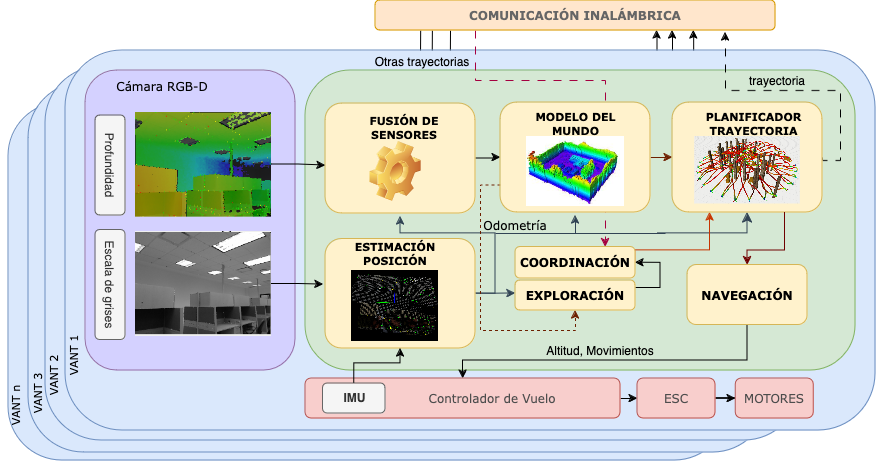
\includegraphics[width=\linewidth]{images/arquitectura}\\
\begin{figure}[h]
\centering
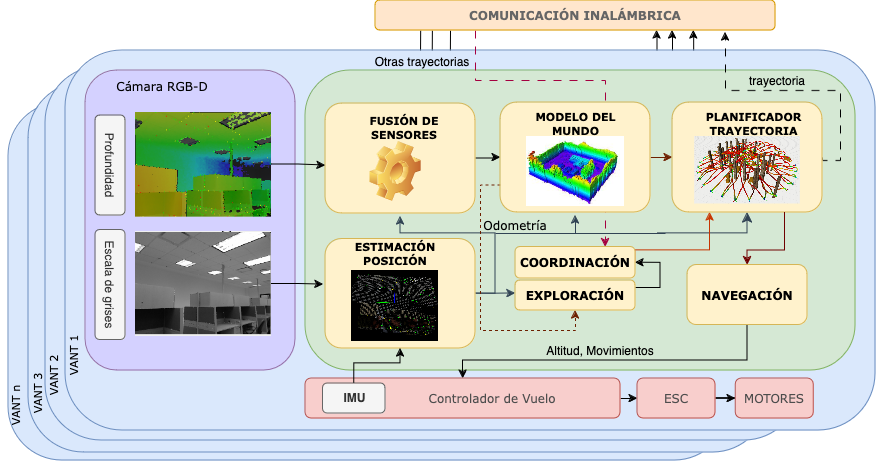
\includegraphics[width=0.8\textwidth]{images/arquitectura}\\
\caption{Arquitectura de la solución propuesta}
\end{figure}

\subsection*{Sistema de percepción}

Al hacer uso del simulador dinámico usado en el trabajo de \citeauthor{RACER2022} y \citeauthor{BARTOLOMEI2023} que utilizan la odometría de referencia de los VANTS, suponiendo que cada agente está equipado con una
cámara de profundidad que mira hacia adelante cuya resolución es 640x480px y un campo de visión de 80ºx60º.

\subsection*{Estimación de posición}
La estimación hace uso de la técnica descrita en el trabajo \citeauthor{OMNI2022}, que ayuda a la localización del VANT y los demás miembros del equipo manteniendo un mismo marco de referencia.

\subsection*{Fusión de sensores}
La función de sensores ayuda a que en el paso previo, se puedan obtener las posiciones aproximadas del equipo de VANTS. Los valores de odometría y el ángulo de inclinación, se fusionan con los datos obtenidos por una nube de puntos.

\subsection*{Representación del mundo}
Una vez conocida la estimación de posición, cada VANT es capaz de intercambiar y actualizar su base de conocimiento para una toma de decisiones informada.

\subsection*{Exploración}
La exploración se basa en el concepto de fronteras propuesto por \citeauthor{YAMAUCHI1997}, debido a que mantiene una lista de fronteras activas cada VANT puede contar con una copia y actualizarla durante su ejecución.

\subsection*{Coordinación}
La coordinación se ofertará después de resolver el problema de asignación que minimicen el tiempo de traslado.

\subsection*{Planificador de trayectorias}
Dentro del planificador, se propone el uso y mantenimiento de un diagrama de Voronoi en 3D, qué, a medida del conocimiento del medio ambiente gracias al sistema de percepción, se podrán suavizar los puntos generando una curva de bezier respecto al punto que el VANT deba trasladarse.

\subsection*{Navegación}
Un enfoque reactivo nos ayuda en aprovechar las velocidades que nuestro VANT puede navegar analizando los obstáculos. De forma que la velocidad se irá reduciendo en base a que la velocidad relacionada al error de detectar un objeto.

Bajo ese comportamiento se podrá acelerar en espacios abiertos y navegar con cuidado cuando se aproxime a zonas estrechas y angostas.

\section{Máquina de estados para un VANT}

Para una mayor comprensión y control de los posibles estados que los VANTS pueden tomar
en las tareas de exploración se abstraen como posibles acciones que deba tomar respecto
al estado en que se encuentre.

\subsection*{Inicialización}

La inicialización constará en todos los procesos antes de comenzar la exploración:
\begin{itemize}\setlength{\itemsep}{-1mm}
\item Situar a los VANTS en su punto inicial conocido.
\item Hacer que los VANTS esperen el cambio de estado para iniciar la exploración.
\end{itemize}

\subsection*{Esperando comenzar exploración}

En este estado, los VANTS esperarán iniciar la exploración manteniendo el vuelo en el punto de inicio.
Una vez alcanzando este estado, se planifica una trayectoria hacia la frontera cercana.
\subsection*{Planeación trayectoria}

Al mantener una representación del medio ambiente, sirve de ayuda para generar una trayectoria que nos aproxime a los puntos de interés.

\subsection*{Publicar trayectoria}

Notificar la trayectoria una vez que se haya validado que existe un camino. Para ello se hace uso del algoritmo A* 

\subsection*{Ejecución trayectoria}

Al contar con una trayectoria que me guia hacia el próximo punto a alcanzar y con ayuda del planificador local que nos permita resolver los problemas de colisiones.


\subsection*{Terminación}

Una vez agotada la lista de fronteras a explorar, el proceso de exploración habrá llegado a su fin.
No se considera que los VANTS regresen al punto inicial, ya que habrán completado el principal objetivo de proporcionar el mapa.

\section{Aplicación de nodos en ROS}

Los nodos en ROS se representan como un grafo dirigido en base a los mensajes que los nodos puedan generar, cada nodo corre en paralelo y tiene su propio ciclo de vida.

\begin{figure}[h]
\centering
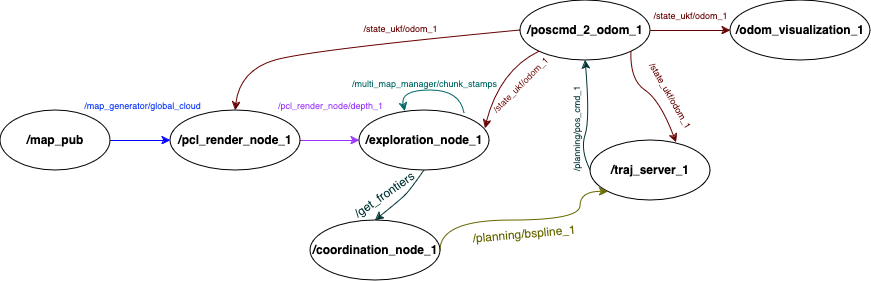
\includegraphics[width=0.98\textwidth]{images/ros_nodes}
\caption{Arquitectura de la solución propuesta}
\end{figure}

\subsection*{Nodo map pub}
La creación del mapa, a partir de un archivo obtenido mediante un sensor capaz de almacenar una nube de puntos.
En nuestro caso, hacemos uso de una cámara kinect v1 y el software RTABMAP para grabar un recorrido a una superficie en interiores que nos ayudará en la propuesta de ciertas geometrias para la tarea de exploración.

\subsection*{Nodo pcl render node 1}
La actualización en base a la posición del VANT, el nodo pcl render node 1, nos arrojará la información en base a las capacidades del campo de visión del VANT.
En nuestro caso, las imágenes de profundidad son de 4.5 m..

\subsection*{Nodo poscmd 2 odom 1}
Conversión del comando de posiciones a valores de odometria de un VANT.

\subsection*{Nodo exploration node 1}

La lógica de exploración se realiza en el nodo de exploración, gracias a la versatilidad de los archivos tipo launch dentro de ROS, permite la creación de diversos nodos respecto a la cardinalidad de agentes en nuestro sistema.

\subsection*{Nodo coordination node 1}

Adoptamos una coordinación descentralizada, donde los agentes intercambian información de su mapa, próximos destinos a cubrir.
Con el objetivo de asignar y repartir las áreas de exploración y construir la representación del medio ambiente de forma colaborativa.

\subsection*{Nodo traj server 1}
Además de la planificación inicial de las trayectorias, el nodo de trayectorias también supervisa continuamente el progreso de los UAV durante la misión. Esto implica ajustar las trayectorias en tiempo real para adaptarse a cambios en el entorno, como la detección de obstáculos móviles o la aparición de nuevas áreas de interés. Esta capacidad de reacción en tiempo real es fundamental para garantizar la seguridad y el éxito de la misión, especialmente en entornos dinámicos y cambiantes.

\subsection*{Nodo odom visualization 1}

El nodo de visualización muestra los datos en tiempo real procedentes de cada uno de los VANTS en RVIZ. Y nos permite conocer lo que está sucediendo en el área de exploración en cualquier momento.
La visualización de los objetos y las fronteras en la simulación se actualizan en el nodo odom visualization 1, actualizando los valores conforme la exploración avanza.
